%%% Beamer slideshow
\documentclass[aspectratio=169]{beamer}

\usepackage{natbib,amsmath,amssymb,graphicx}
\usepackage{booktabs}
\usepackage{multirow}
\usepackage{hyperref}
\usepackage{multicol}
\usepackage{array}
\usepackage{bbm}
\usepackage{bm}

\newcolumntype{L}[1]{>{\raggedright\arraybackslash}p{#1}}
\newcolumntype{C}[1]{>{\centering\arraybackslash}p{#1}}
\newcolumntype{R}[1]{>{\raggedleft\arraybackslash}p{#1}}

\graphicspath{{../Figures/Figures_v3/}{../Figures/Figures_Retirement/}{../Figures/DurableModel/}}

\newcommand{\Ret}{\mathrm{Ret}}
\newcommand{\eff}{\varepsilon}
\newcommand{\goth}[1]{\mathcal{#1}}
\newcommand{\E}{\mathbb{E}}

\mode<presentation>
{
	\usetheme{CambridgeUS}
	\usecolortheme{default}
	\usefonttheme{default}
	\setbeamertemplate{navigation symbols}{}
	\mode<beamer>{\setbeamertemplate{blocks}[rounded][shadow=true]}
	\setbeamertemplate{caption}[numbered]
	\useoutertheme{infolines}
	\useoutertheme[subsection=false]{miniframes}
}

\title[Search Smooths DC Problems]{Search Smooths Discontinuities in\\ Discrete/Continuous Problems}
\author[Carroll, Iskhakov, Khan, Monninger]{Christopher D.\ Carroll \and Fedor Iskhakov \and Shujaat Khan \and Adrian Monninger}
\institute[]{JHU \and Stony Brook \and IMF \and Texas A\&M}
\date{\today}

\begin{document}

%%% Title slide
\begin{frame}[plain]
	\titlepage
\end{frame}


%============================================================
\section{Introduction}
%============================================================

%%% Introduction
\begin{frame}[label = Introduction]
	\frametitle{Discontinuities break EGM in discrete--continuous problems}
	\textbf{Problem:}
	\begin{itemize}
		\item EGM is efficient when the choice is continuous and the value function is concave
		\item With discrete \emph{and} continuous choices, the Euler equation is only necessary
		\item Kinks in $V$ and jumps in the policy create non-monotonic endogenous grids
		\item[$\to$] suboptimal EGM points; kinks propagate under backward induction
	\end{itemize}
	\vspace{0.75em}
	\pause
	\textbf{Standard fix:} Extreme Value Type~I taste shocks
	\begin{itemize}
		\item McFadden (discrete choice); Iskhakov et al.\ (2017) for consumption--saving DC-EGM
		\item Smooths $V$ and marginal utilities, but randomizes the discrete outcome
	\end{itemize}
	\vspace{0.75em}
	\pause
	\textbf{This paper:} directed search + price dispersion
	\begin{itemize}
		\item Search effort governs the probability of switching the discrete state
		\item Price (or account) draws rationalize when the switch is exercised
		\item Smoothness is part of the agent's economic problem---not only a numerical trick
	\end{itemize}
\end{frame}

%%% Reason why search and price vs taste shocks
\begin{frame}[label = WhySearch]
	\frametitle{Why search and prices instead of taste shocks?}
	\begin{enumerate}\setlength\itemsep{0.9em}
		\item \textbf{Local to the threshold}\\
		Search affects agents near S,s (or work--retire) bands; taste shocks put mass on dominated branches far from indifference
		\item \textbf{Microfounded and measurable}\\
		Search intensity $\varepsilon^\ast\in[0,1]$ maps to expected search duration --- observable in microdata\\
		Taste-shock scale $\sigma_\varepsilon$ is hard to interpret (match far-from-threshold adjusters or iMPCs)
		\item \textbf{Compatible with permanent-income normalization}\\
		Search costs can scale with permanent income; additive EV shocks typically cannot $\Rightarrow$ extra state
	\end{enumerate}
	\vspace{0.75em}
	\pause
	\textbf{Complementarity:} search alone is one-sided; price dispersion (or small taste shocks) delivers uniform smoothness around discontinuities
\end{frame}


%============================================================
\section{Retirement model}
%============================================================

%%% Retirement problem: basic problem math
\begin{frame}[label = RetBasic]
	\frametitle{Retirement model: environment}
	\begin{itemize}
		\item Utility: $u(c_t,d_t,\eff_t)=\log(c_t)-\delta d_t-\theta(\eff_t)$
		\item Search cost: $\theta(\eff_t)=\sigma_s\big(\eff_t+(1-\eff_t)\log(1-\eff_t)\big)$
		\item Discrete state: work ($d_t=1$) or retire ($d_t=0$), retirement absorbing
		\item Budget: $M_t=R A_{t-1}+y_t d_{t-1}$, with $y_t=y\eta_t$, $\eta_t$ mean-one lognormal
		\item Option to retire arrives with probability $P_1(\eff_{t-1})=(1-\eff_{t-1})p+\eff_{t-1}$
	\end{itemize}
	\vspace{0.5em}
	\pause
	\textbf{Retiree (absorbing):}
	\begin{align*}
		V_t^{\Ret}(M_t)=\max_{0\le c_t\le M_t}\big\{\log(c_t)+\beta V_{t+1}^{\Ret}(R A_t)\big\}
	\end{align*}
\end{frame}

\begin{frame}[label = RetWorker]
	\frametitle{Retirement model: worker's problem}
	Must-work branch $\mathcal{D}_t=\{W\}$:
	\begin{align*}
		V_t(M_t,\{W\},\xi_t)
		&= \xi_t \max_{\substack{0\le c_t\le M_t\\ 0\le\eff_t\le 1}}
		\Big\{u(c_t,1,\eff_t)
		+\beta P_1(\eff_t)\,\goth{V}_t^1(A_t)
		+\beta P_2(\eff_t)\,\goth{V}_t^2(A_t)\Big\}
	\end{align*}
	\pause
	With option $\mathcal{D}_t=\{R,W\}$:
	\begin{align*}
		V_t(M_t,\{R,W\},\xi_t)
		= \max\big\{V_t^{\Ret}(M_t);\; V_t(M_t,\{W\},\xi_t)\big\}
	\end{align*}
	\vspace{0.25em}
	Optimal effort (after consumption):
	\begin{align*}
		\eff_t^\ast
		= 1-\exp\!\left(-\frac{\beta(1-p)}{\sigma_s}\big(\goth{V}_t^1(A_t)-\goth{V}_t^2(A_t)\big)\right)
	\end{align*}
\end{frame}

%%% Retirement problem: taste shocks
\begin{frame}[label = RetTaste]
	\frametitle{Retirement: multiplicative log-normal taste shocks}
	\begin{itemize}
		\item $\xi_t\sim\mathcal{N}(-\sigma_\xi^2/2,\sigma_\xi^2)$ scales the value of working
		\item Unlike EV Type~I (Iskhakov et al.), these shocks are discretized and feed into search effort
		\item Alone: expand the region where agents search around discontinuities
	\end{itemize}
	\vspace{0.5em}
	\begin{columns}[T]
		\begin{column}{0.48\textwidth}
			\centering
			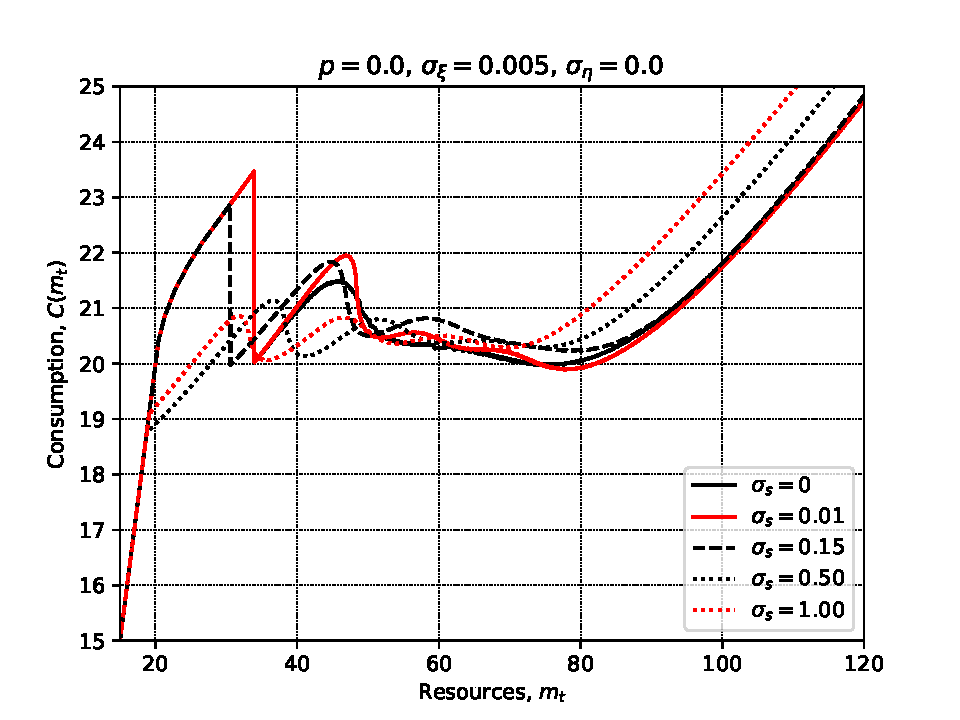
\includegraphics[width=\linewidth]{p0_xi0p005_eta0.pdf}\\
			{\scriptsize $\sigma_\xi=0.005$, $p=0$}
		\end{column}
		\begin{column}{0.48\textwidth}
			\centering
			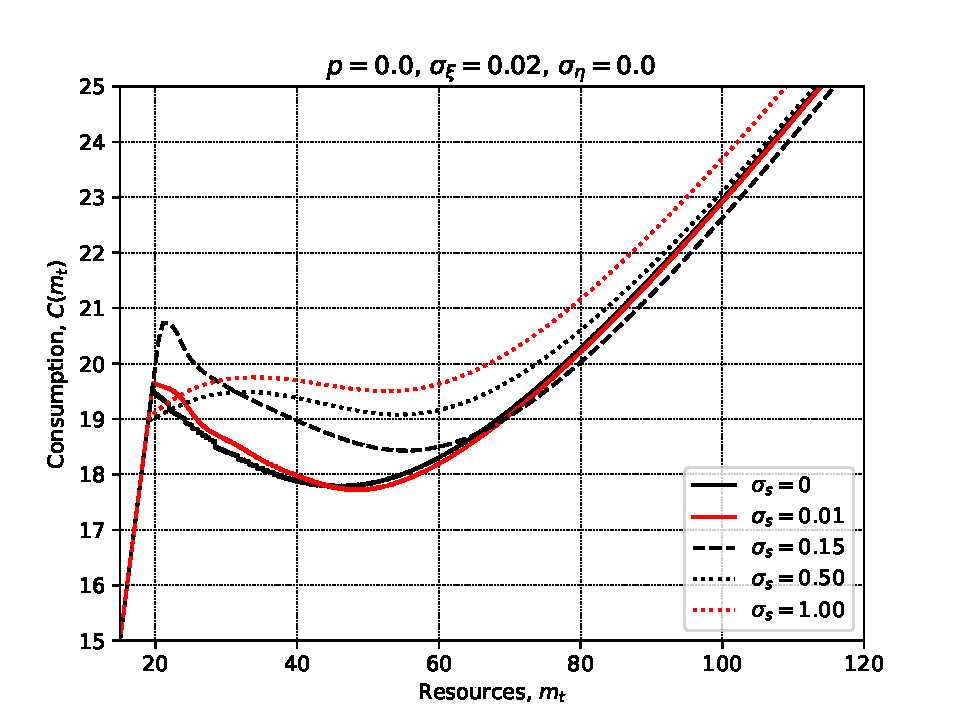
\includegraphics[width=\linewidth]{p0_xi0p02_eta0.pdf}\\
			{\scriptsize $\sigma_\xi=0.02$, $p=0$}
		\end{column}
	\end{columns}
\end{frame}

%%% Retirement problem: Search
\begin{frame}[label = RetSearch]
	\frametitle{Retirement: directed search smooths (asymmetrically)}
	\begin{itemize}
		\item $p=1$: option arrives for free $\Rightarrow$ $\eff^\ast=0$, no smoothing from $\sigma_s$
		\item $p=0$: must search to retire $\Rightarrow$ larger $\sigma_s$ smooths to the \emph{right} of kinks
		\item Low-$M$ workers optimally set $\eff^\ast=0$ (plan to keep working)
	\end{itemize}
	\vspace{0.35em}
	\begin{columns}[T]
		\begin{column}{0.48\textwidth}
			\centering
			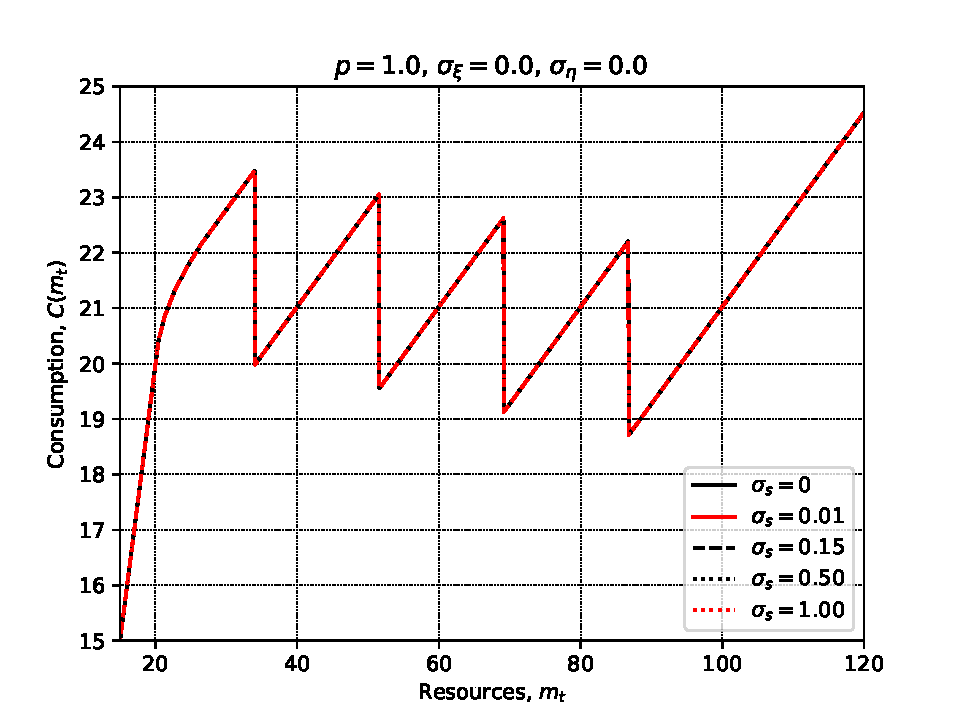
\includegraphics[width=\linewidth]{p1_xi0_eta0.pdf}\\
			{\scriptsize $p=1$: no search motive}
		\end{column}
		\begin{column}{0.48\textwidth}
			\centering
			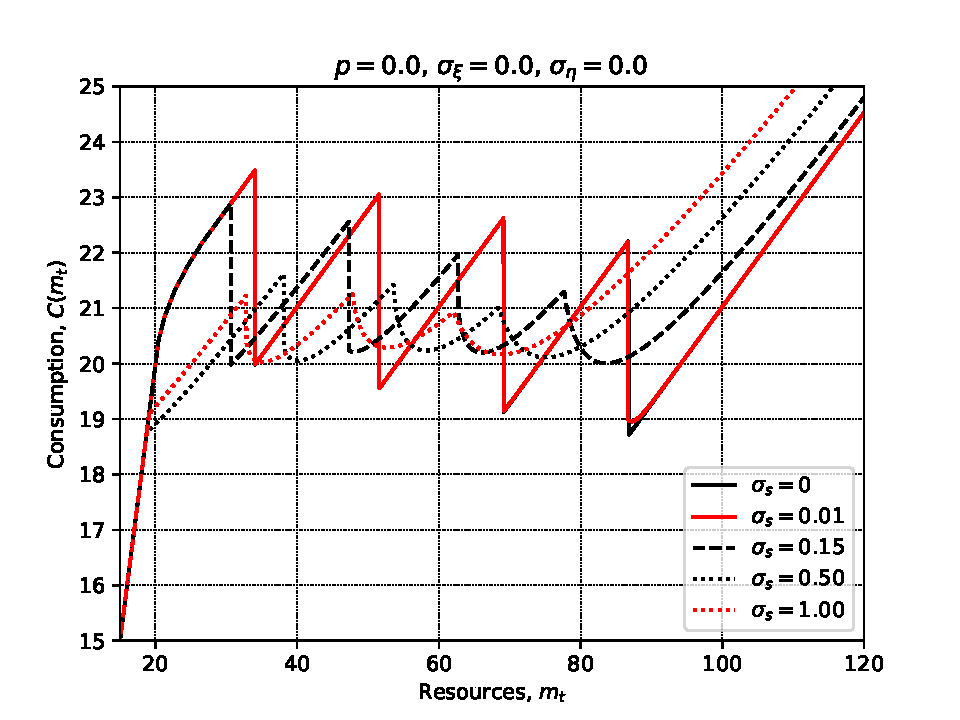
\includegraphics[width=\linewidth]{p0_xi0_eta0.pdf}\\
			{\scriptsize $p=0$: search smooths right of kinks}
		\end{column}
	\end{columns}
\end{frame}

\begin{frame}[label = RetSearchTaste]
	\frametitle{Retirement: search + taste shocks $\Rightarrow$ uniform smoothness}
	\begin{columns}[T]
		\begin{column}{0.48\textwidth}
			\centering
			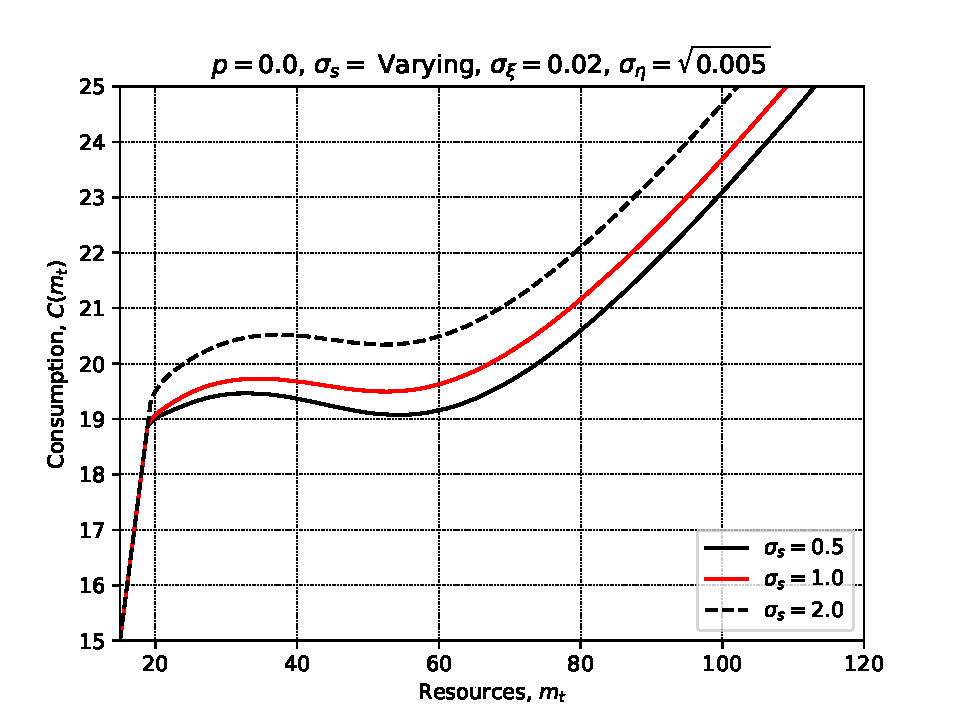
\includegraphics[width=\linewidth]{VaryS.pdf}\\
			{\scriptsize Raising $\sigma_s$ shifts $c$ \textbf{up}}
		\end{column}
		\begin{column}{0.48\textwidth}
			\centering
			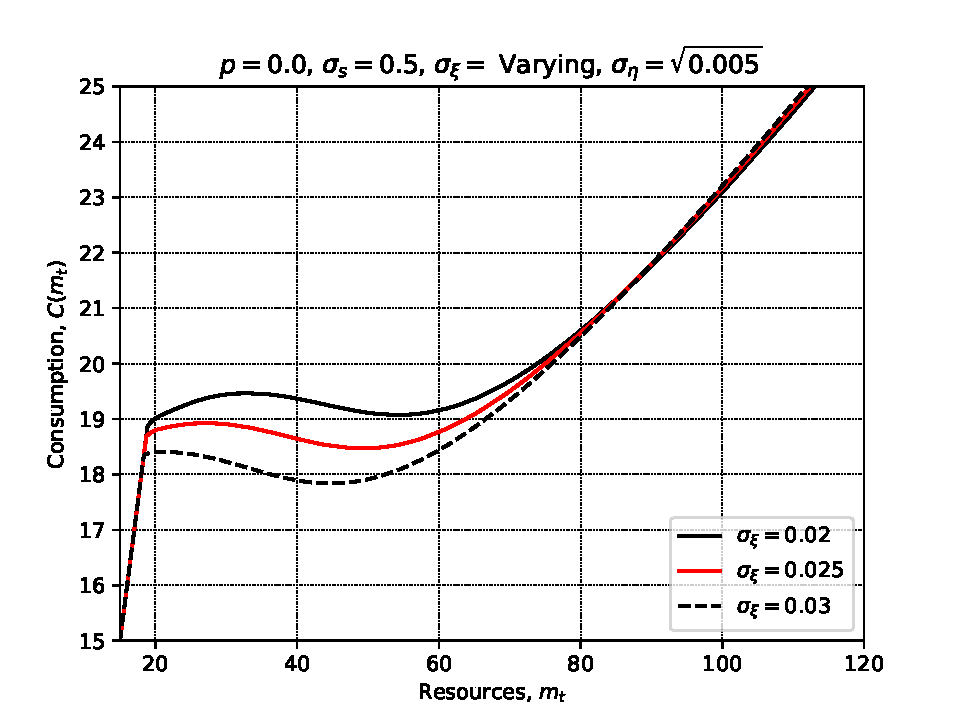
\includegraphics[width=\linewidth]{VaryXi.pdf}\\
			{\scriptsize Raising $\sigma_\xi$ shifts $c$ \textbf{down}}
		\end{column}
	\end{columns}
	\vspace{0.5em}
	\begin{itemize}
		\item Search / lower $p$: fewer successful switches $\Rightarrow$ more expected work years $\Rightarrow$ higher $c$
		\item Larger taste (or income) shocks: precautionary saving $\Rightarrow$ lower $c$
		\item Same smoothness goal, opposite level shifts
	\end{itemize}
\end{frame}

%%% Retirement problem: Price dispersion
\begin{frame}[label = RetPrice]
	\frametitle{Retirement: stochastic account realizations}
	After receiving the option, draw rejectable retirement wealth factor $\phi_t$:
	\begin{align*}
		\log\phi_t\sim\mathcal{N}\!\big(-\tfrac{\sigma_\phi^2}{2},\sigma_\phi^2\big),\quad
		\tilde M_t=\phi_t M_t,\quad
		V_t(M_t,\phi_t)=\max\big\{V_t^{\Ret}(\phi_t M_t),\,V_t^{W}(M_t)\big\}
	\end{align*}
	Ex-ante value $\bar V_t(M_t)=\E_{\phi_t}[V_t(M_t,\phi_t)]$ replaces a single threshold $M^\ast$ by a family $M^\ast(\phi)$.
	\vspace{0.35em}
	\begin{columns}[T]
		\begin{column}{0.48\textwidth}
			\centering
			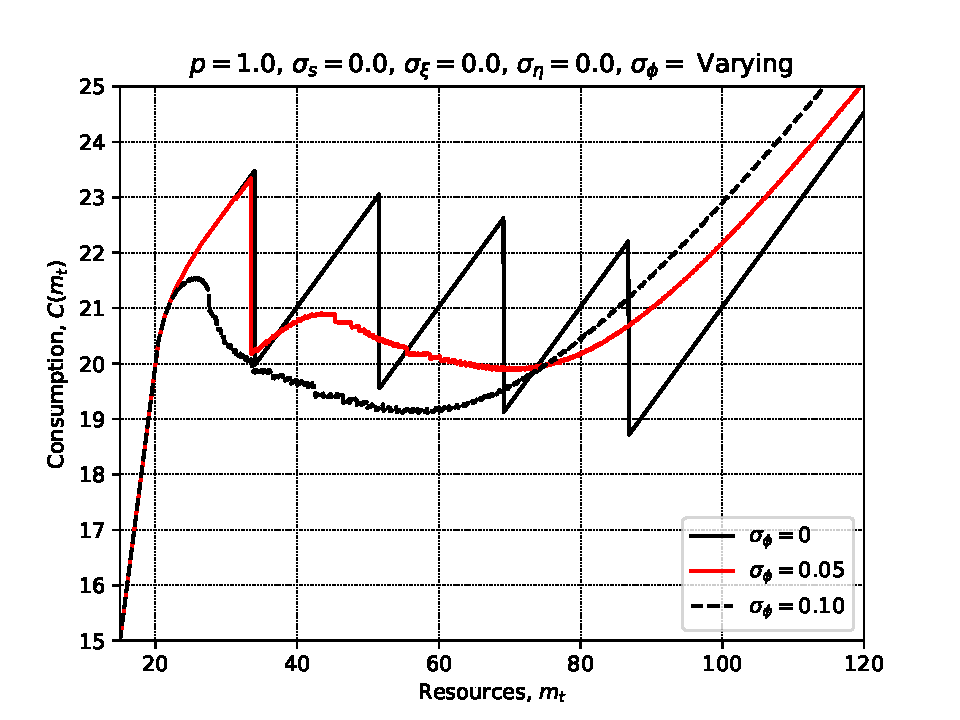
\includegraphics[width=\linewidth]{VaryPhi.pdf}\\
			{\scriptsize Larger $\sigma_\phi$ smooths more}
		\end{column}
		\begin{column}{0.48\textwidth}
			\centering
			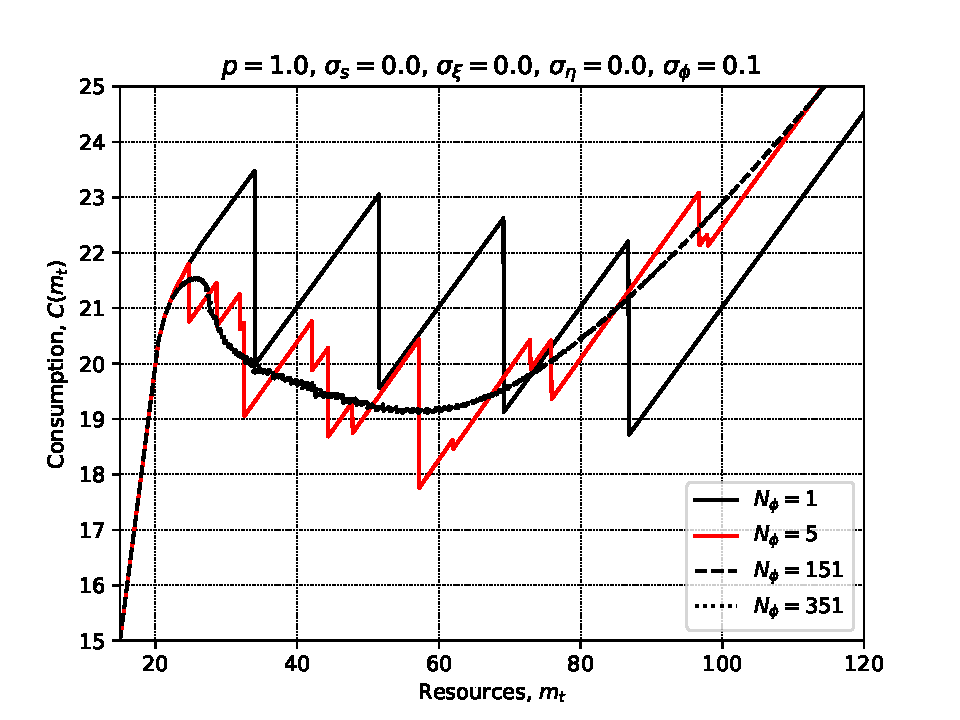
\includegraphics[width=\linewidth]{VaryPhiCount.pdf}\\
			{\scriptsize Need enough $\phi$-nodes}
		\end{column}
	\end{columns}
\end{frame}

%%% Retirement problem: Search and price together
\begin{frame}[label = RetSearchPrice]
	\frametitle{Retirement: search and account dispersion together}
	\begin{itemize}
		\item Search governs \emph{whether} a draw arrives; $\phi_t$ is the \emph{content} of the draw
		\item Complements: option value of $\phi$ raises $\goth{V}^1-\goth{V}^2$ $\Rightarrow$ more search
	\end{itemize}
	\vspace{0.35em}
	\begin{columns}[T]
		\begin{column}{0.48\textwidth}
			\centering
			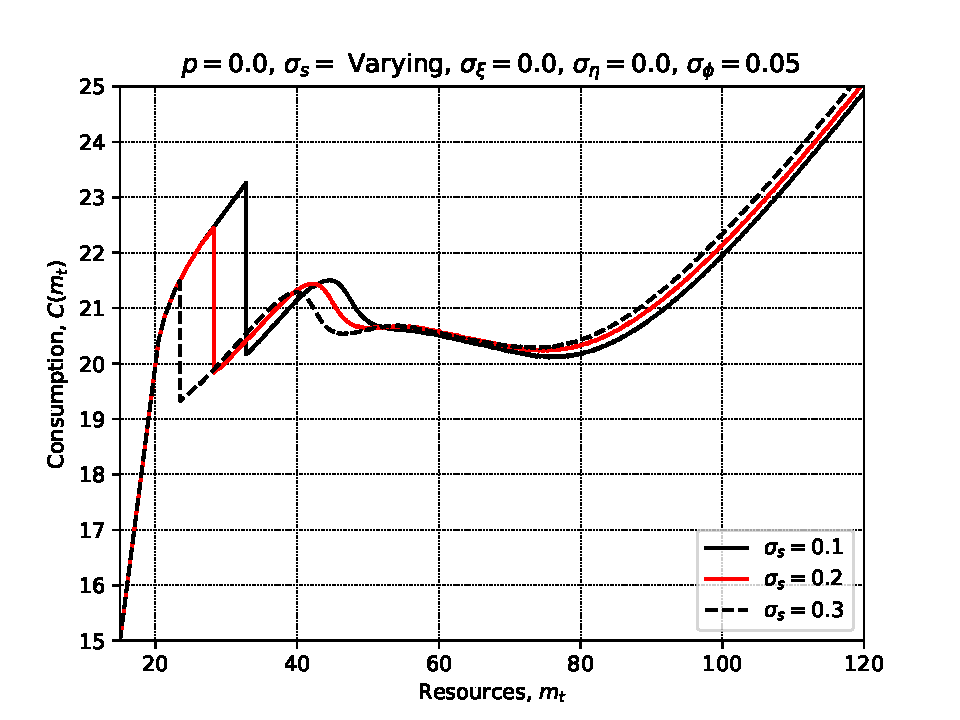
\includegraphics[width=\linewidth]{SearchPhi_VaryS.pdf}\\
			{\scriptsize Vary search given $\phi$}
		\end{column}
		\begin{column}{0.48\textwidth}
			\centering
			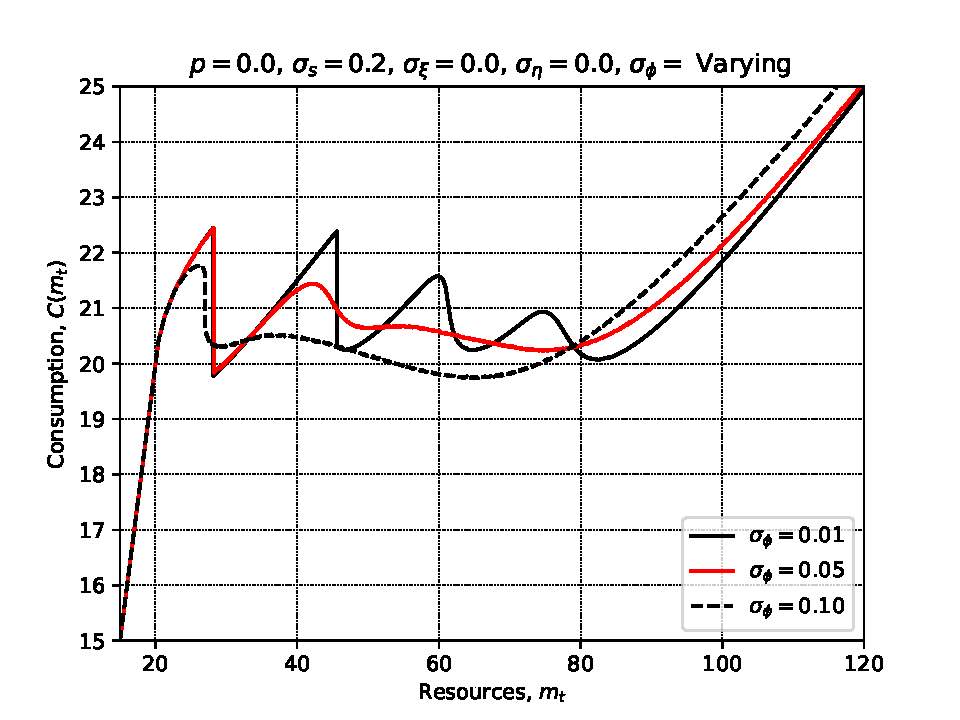
\includegraphics[width=\linewidth]{SearchPhi_VaryPhi.pdf}\\
			{\scriptsize Vary $\sigma_\phi$ given search}
		\end{column}
	\end{columns}
\end{frame}


%============================================================
\section{Durable model}
%============================================================

%%% Durablemodel: basic problem math
\begin{frame}[label = DurBasic]
	\frametitle{Durable model: keep vs adjust}
	\begin{align*}
		u(c_t,d_t)&=\frac{(c_t^\alpha d_t^{1-\alpha})^{1-\rho}}{1-\rho},\qquad
		\ell_t=m_t+(1-\tau)n_t
	\end{align*}
	Hard maximum:
	\begin{align*}
		v_t(m_t,n_t)=\max\big\{v_t^{\mathrm{keep}}(m_t,n_t),\; v_t^{\mathrm{adj}}(\ell_t)\big\}
	\end{align*}
	\pause
	\begin{columns}[T]
		\begin{column}{0.48\textwidth}
			{\small Keeper:}
			\begin{align*}
				v_t^{\mathrm{keep}}&=\max_{c_t} u(c_t,n_t)+\beta\E_t[v_{t+1}]\\
				a_t&=m_t-c_t\ge 0,\quad d_t=n_t
			\end{align*}
		\end{column}
		\begin{column}{0.48\textwidth}
			{\small Adjuster:}
			\begin{align*}
				v_t^{\mathrm{adj}}&=\max_{c_t,d_t} u(c_t,d_t)+\beta\E_t[v_{t+1}]\\
				a_t&=\ell_t-c_t-d_t\ge 0
			\end{align*}
		\end{column}
	\end{columns}
	\vspace{0.25em}
	Laws of motion: $m_{t+1}=\mathcal{R}a_t+\theta_{t+1}$, $n_{t+1}=(1-\delta)d_t$
\end{frame}

\begin{frame}[label = DurBaselineFig]
	\frametitle{Baseline hard max: S,s bands and discontinuous policies}
	\begin{columns}[T]
		\begin{column}{0.48\textwidth}
			\centering
			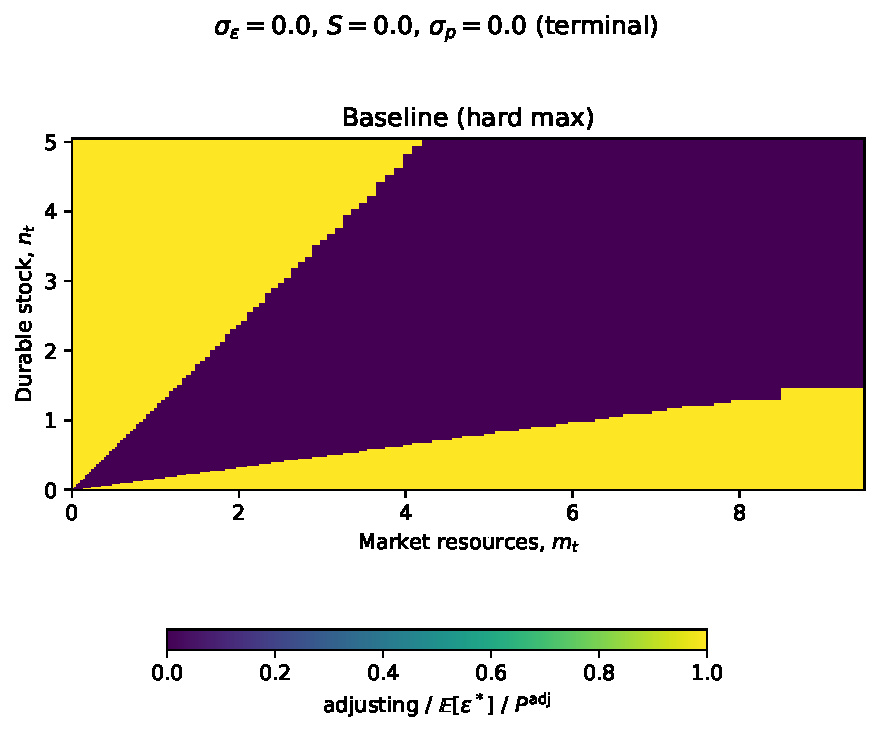
\includegraphics[width=\linewidth]{Baseline_Ss_T.pdf}\\
			{\scriptsize Terminal keep--adjust regions}
		\end{column}
		\begin{column}{0.48\textwidth}
			\centering
			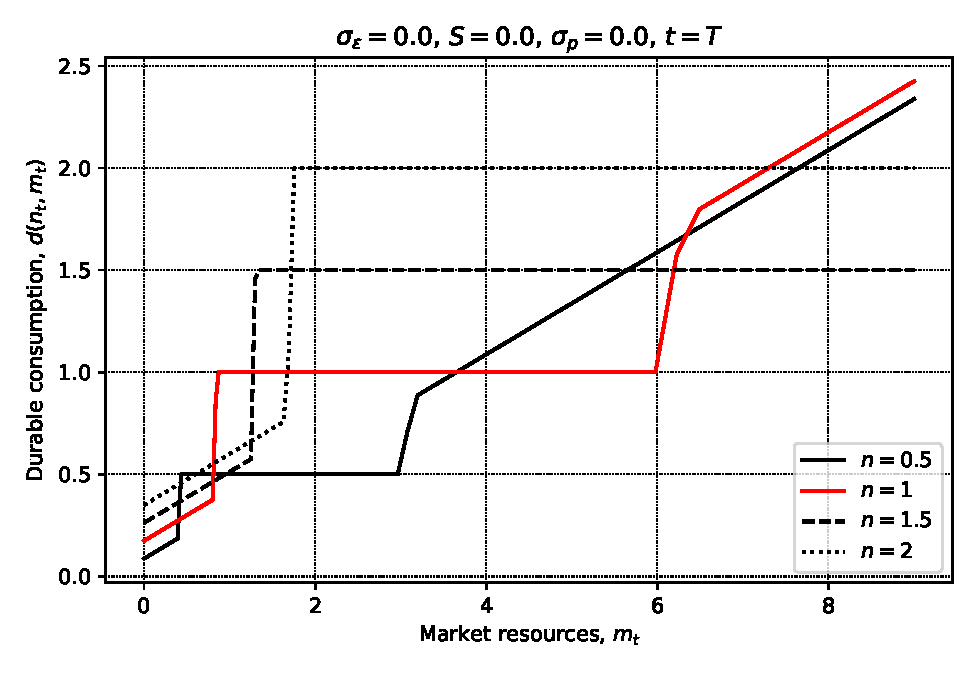
\includegraphics[width=\linewidth]{Baseline_d_T.pdf}\\
			{\scriptsize Combined durable policy}
		\end{column}
	\end{columns}
	\vspace{0.35em}
	\begin{itemize}
		\item Sharp switch $\Rightarrow$ discontinuities; earlier periods inherit next-period switchpoints
		\item Non-convex $\tau$ $\Rightarrow$ FOCs only necessary $\Rightarrow$ need DC-EGM / FUES
	\end{itemize}
\end{frame}

%%% Durablemodel: taste shock problem math
\begin{frame}[label = DurTasteMath]
	\frametitle{Durable model: EV Type~I taste shocks}
	\begin{align*}
		v_t
		&= \sigma_\varepsilon\log\Big(
			\exp\big(v_t^{\mathrm{keep}}/\sigma_\varepsilon\big)
			+\exp\big(v_t^{\mathrm{adj}}/\sigma_\varepsilon\big)
		\Big)
	\end{align*}
	Logit probabilities and mixed policies:
	\begin{align*}
		P_t^{\mathrm{adj}}
		&=\frac{\exp(v_t^{\mathrm{adj}}/\sigma_\varepsilon)}
		{\exp(v_t^{\mathrm{keep}}/\sigma_\varepsilon)+\exp(v_t^{\mathrm{adj}}/\sigma_\varepsilon)},\\
		c_t &= P_t^{\mathrm{keep}}\,c_t^{\mathrm{keep}}+P_t^{\mathrm{adj}}\,c_t^{\mathrm{adj}},\quad
		d_t = P_t^{\mathrm{keep}}\,n_t+P_t^{\mathrm{adj}}\,d_t^{\mathrm{adj}}
	\end{align*}
	\vspace{0.25em}
	\begin{itemize}
		\item Closed form (no taste quadrature); continuous FOCs unchanged
		\item $\sigma_\varepsilon\to 0$ recovers hard max
	\end{itemize}
\end{frame}

%%% Durablemodel: taste shock: SS in terminal period
\begin{frame}[label = DurTasteSS]
	\frametitle{Taste shocks: terminal S,s bands}
	\begin{center}
		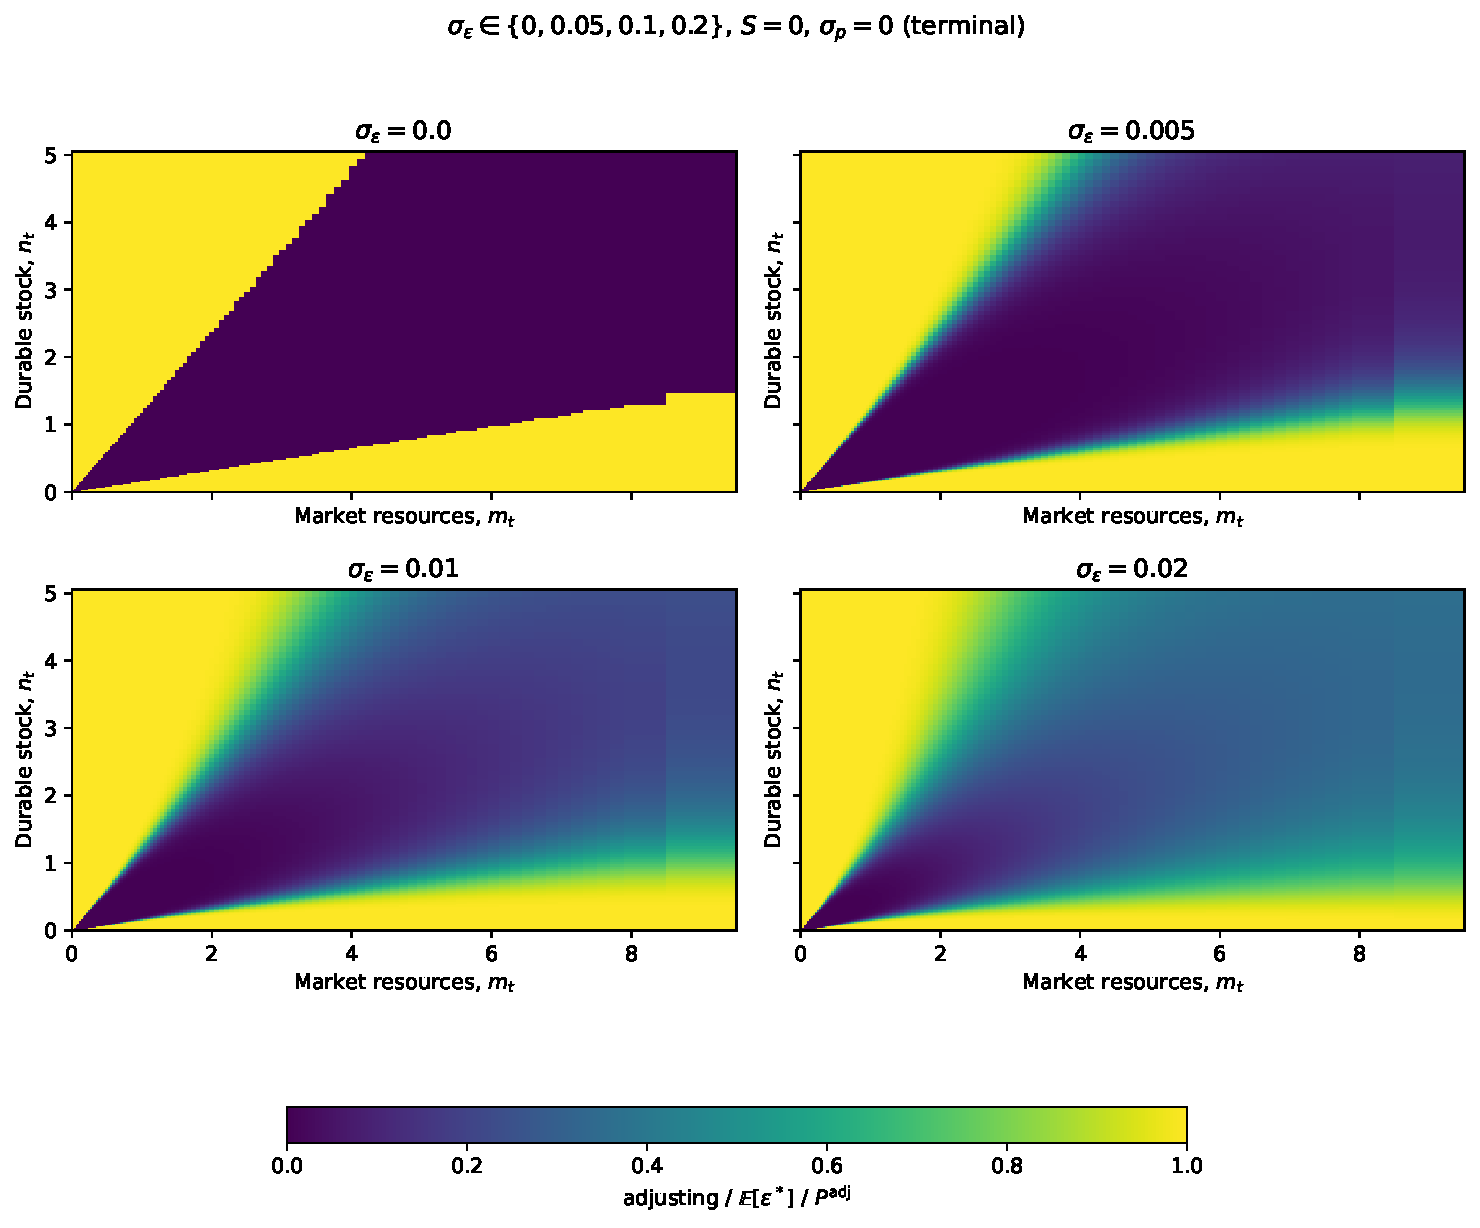
\includegraphics[width=0.72\linewidth]{TasteShock_Ss_T.pdf}
	\end{center}
	\vspace{-0.25em}
	\begin{itemize}
		\item $\sigma_\varepsilon\in\{0,0.05,0.1,0.2\}$: adjustment probability interior near indifference
		\item Combined policies become convex combinations around the band
	\end{itemize}
\end{frame}

%%% Durablemodel: Search problem math
\begin{frame}[label = DurSearchMath]
	\frametitle{Durable model: directed search}
	\begin{align*}
		\sigma(\varepsilon_t)&=S\big[\varepsilon_t+(1-\varepsilon_t)\log(1-\varepsilon_t)\big]\\[0.35em]
		v_t(m_t,n_t)
		&=\max_{\varepsilon_t\in[0,1]}
		\Big[(1-\varepsilon_t)\,v_t^{\mathrm{keep}}
		+\varepsilon_t\,v_t^{\mathrm{adj}}
		-\sigma(\varepsilon_t)\Big]
	\end{align*}
	\vspace{0.35em}
	\begin{itemize}
		\item $\varepsilon_t$: probability of locating a suitable durable this period
		\item $S\to 0$: hard max; $S\to\infty$: never adjusts
		\item Effort chosen before the discrete outcome --- economically local near the band
	\end{itemize}
\end{frame}

%%% Durablemodel: Search: SS in terminal period
\begin{frame}[label = DurSearchSS]
	\frametitle{Search: terminal S,s bands}
	\begin{center}
		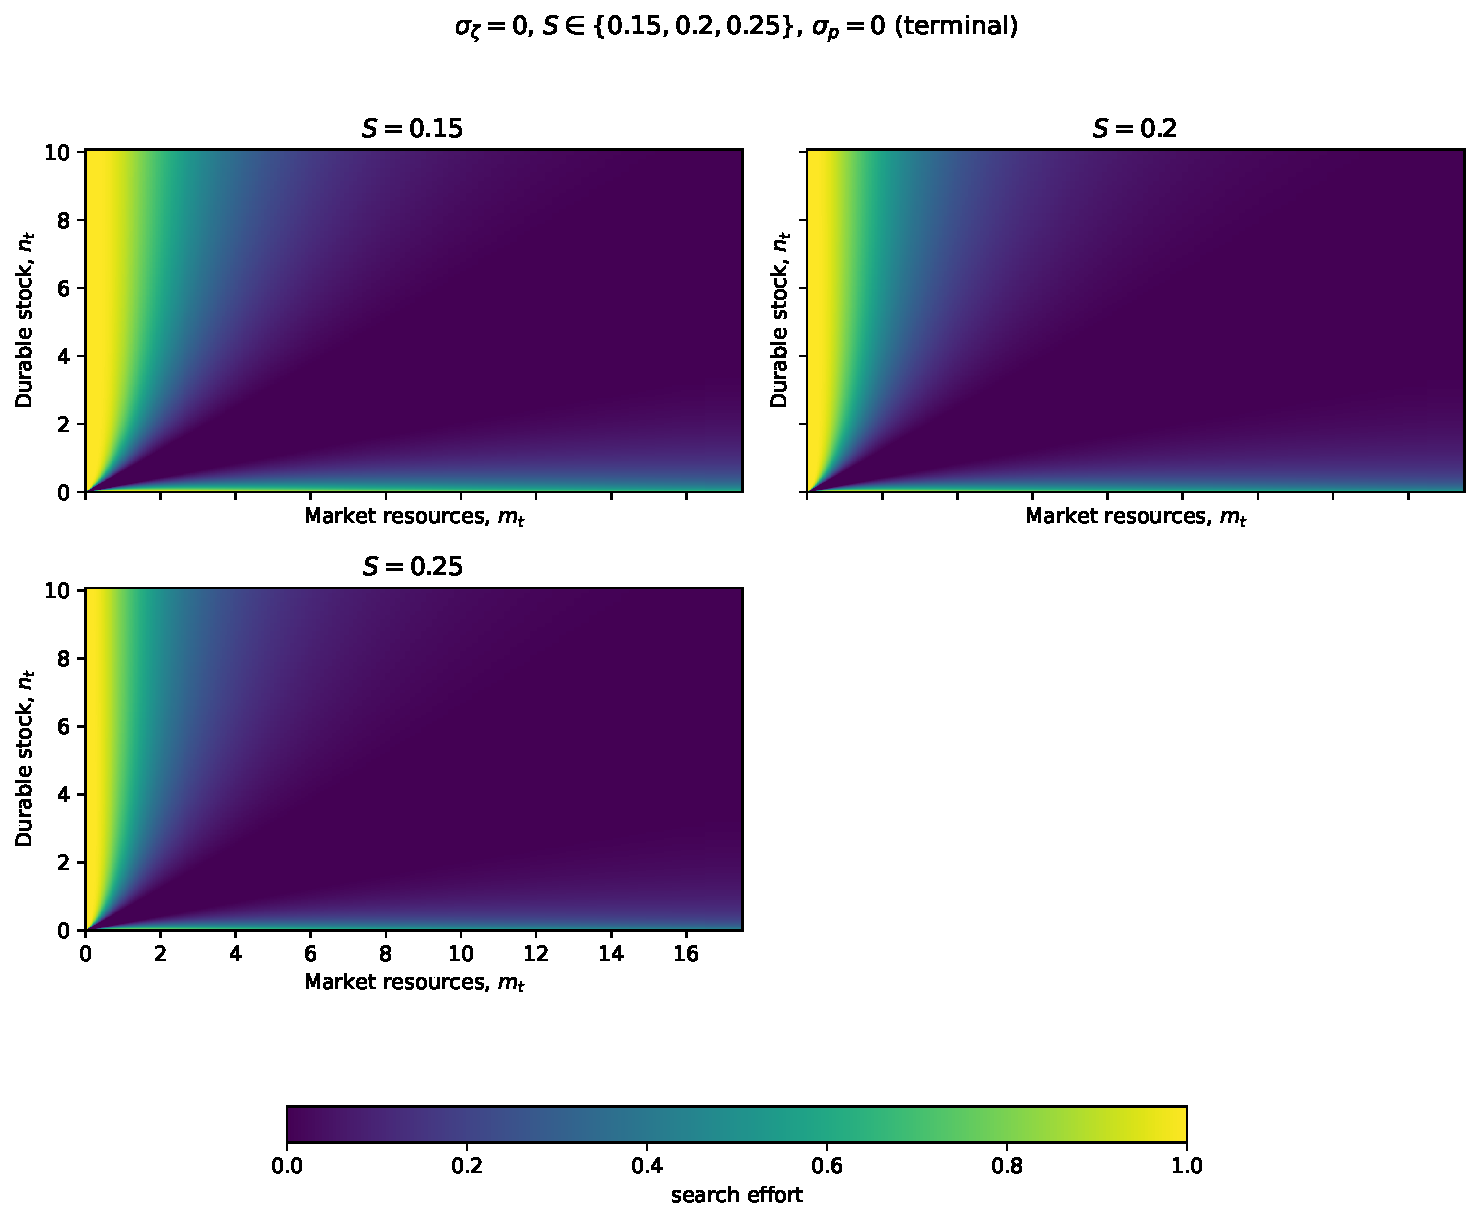
\includegraphics[width=0.72\linewidth]{Search_Ss_T.pdf}
	\end{center}
	\vspace{-0.25em}
	\begin{itemize}
		\item $S\in\{0,0.05,0.1,0.2\}$: small friction already softens the keep--adjust frontier
		\item Comparable visual smoothness to EV taste shocks
	\end{itemize}
\end{frame}

%%% Durablemodel: Price dispersion problem math
\begin{frame}[label = DurPriceMath]
	\frametitle{Durable model: stochastic purchase prices}
	\begin{align*}
		\log p_t&\sim\mathcal{N}\!\big(-\tfrac{\sigma_p^2}{2},\sigma_p^2\big),\quad
		a_t=\ell_t-c_t-p_t\,d_t\ge 0
	\end{align*}
	Price-contingent hard max and ex-ante value:
	\begin{align*}
		v_t(m_t,n_t,p_t)
		&=\max\big\{v_t^{\mathrm{keep}}(m_t,n_t),\;v_t^{\mathrm{adj}}(\ell_t,p_t)\big\}\\
		\bar v_t(m_t,n_t)
		&=\E_{p_t}\big[v_t(m_t,n_t,p_t)\big]
	\end{align*}
	\vspace{0.25em}
	\begin{itemize}
		\item Only \emph{new} durable purchases face $p_t$; liquidation still at rate $1-\tau$
		\item Changes adjuster's continuous FOC in $d_t$ (unlike EV shocks)
		\item Low $p_t$ accepted, high $p_t$ rejected --- softens the extensive margin
	\end{itemize}
\end{frame}

%%% Durablemodel: Price dispersion: SS in terminal period
\begin{frame}[label = DurPriceSS]
	\frametitle{Price dispersion: terminal adjustment regions}
	\begin{center}
		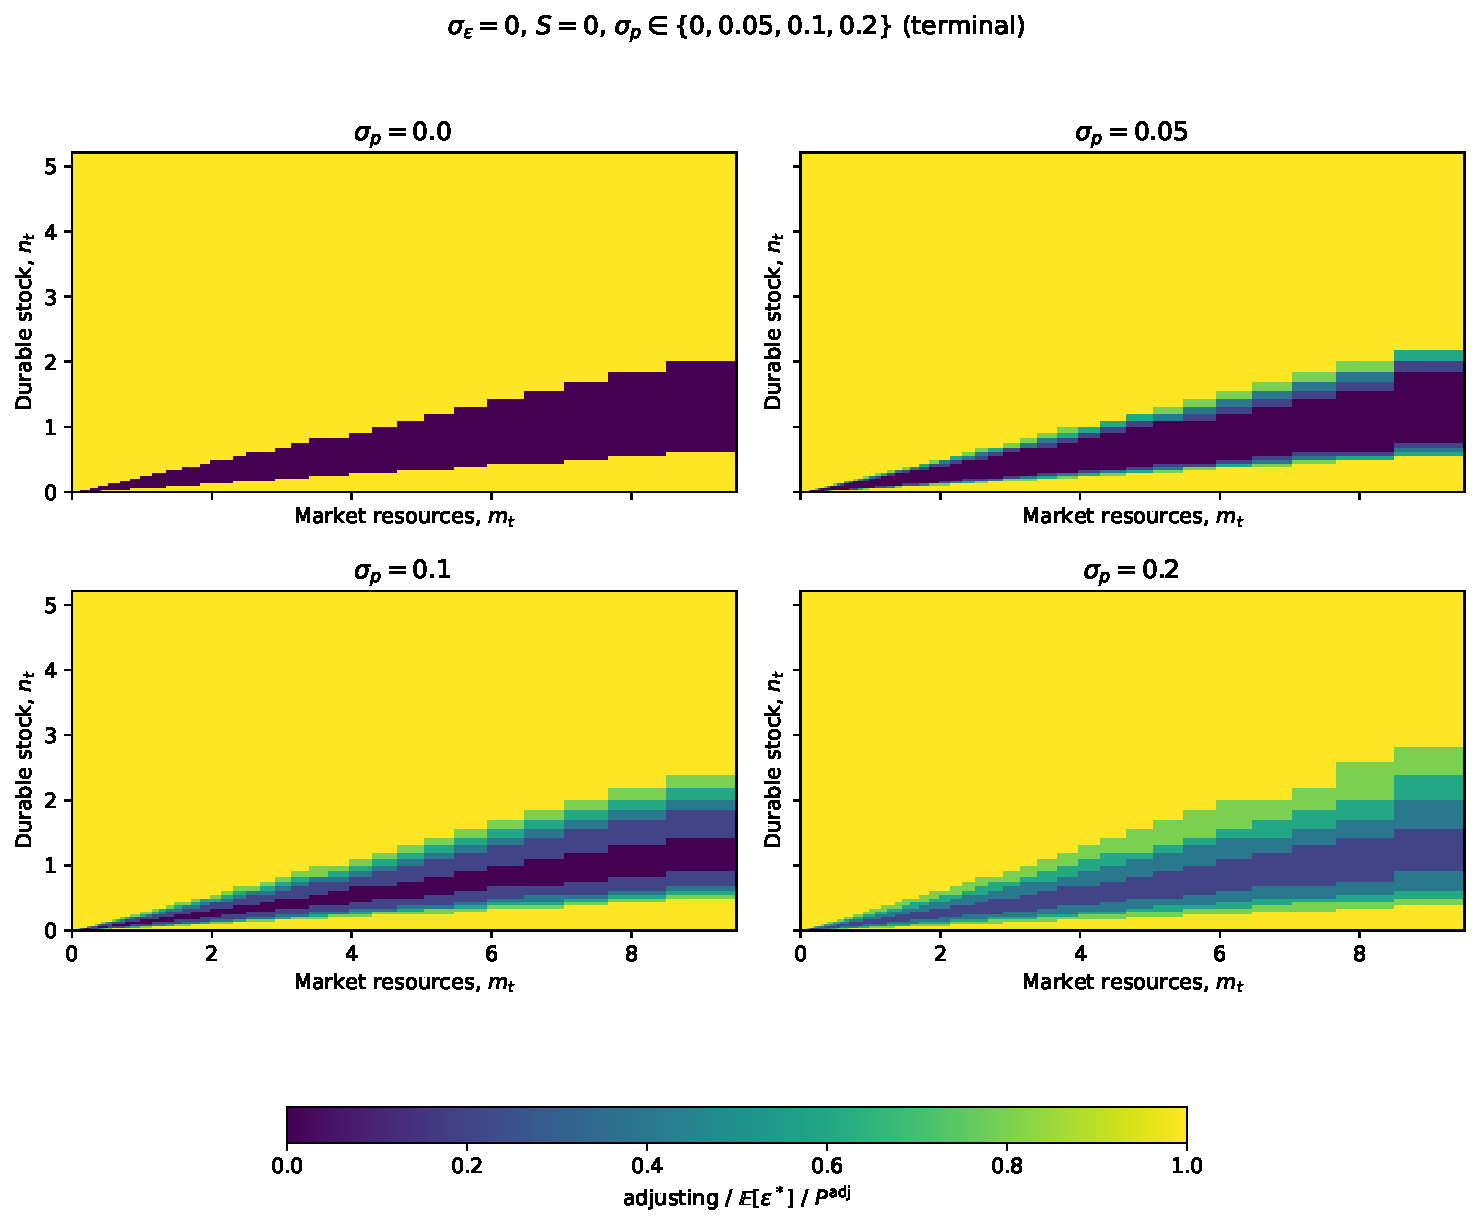
\includegraphics[width=0.78\linewidth]{PriceStd_Ss_T.pdf}
	\end{center}
	\vspace{-0.25em}
	\begin{itemize}
		\item $\sigma_p\in\{0,0.05,0.1,0.2\}$ softens the hard threshold via rejectable offers
		\item Sharp thresholds remain; period-$t$ policies less smooth than taste/search alone
	\end{itemize}
\end{frame}

%%% Durablemodel: Combined non-durable consumption functions
\begin{frame}[label = DurCombinedC]
	\frametitle{Combined nondurable consumption: all channels move together}
	\begin{center}
		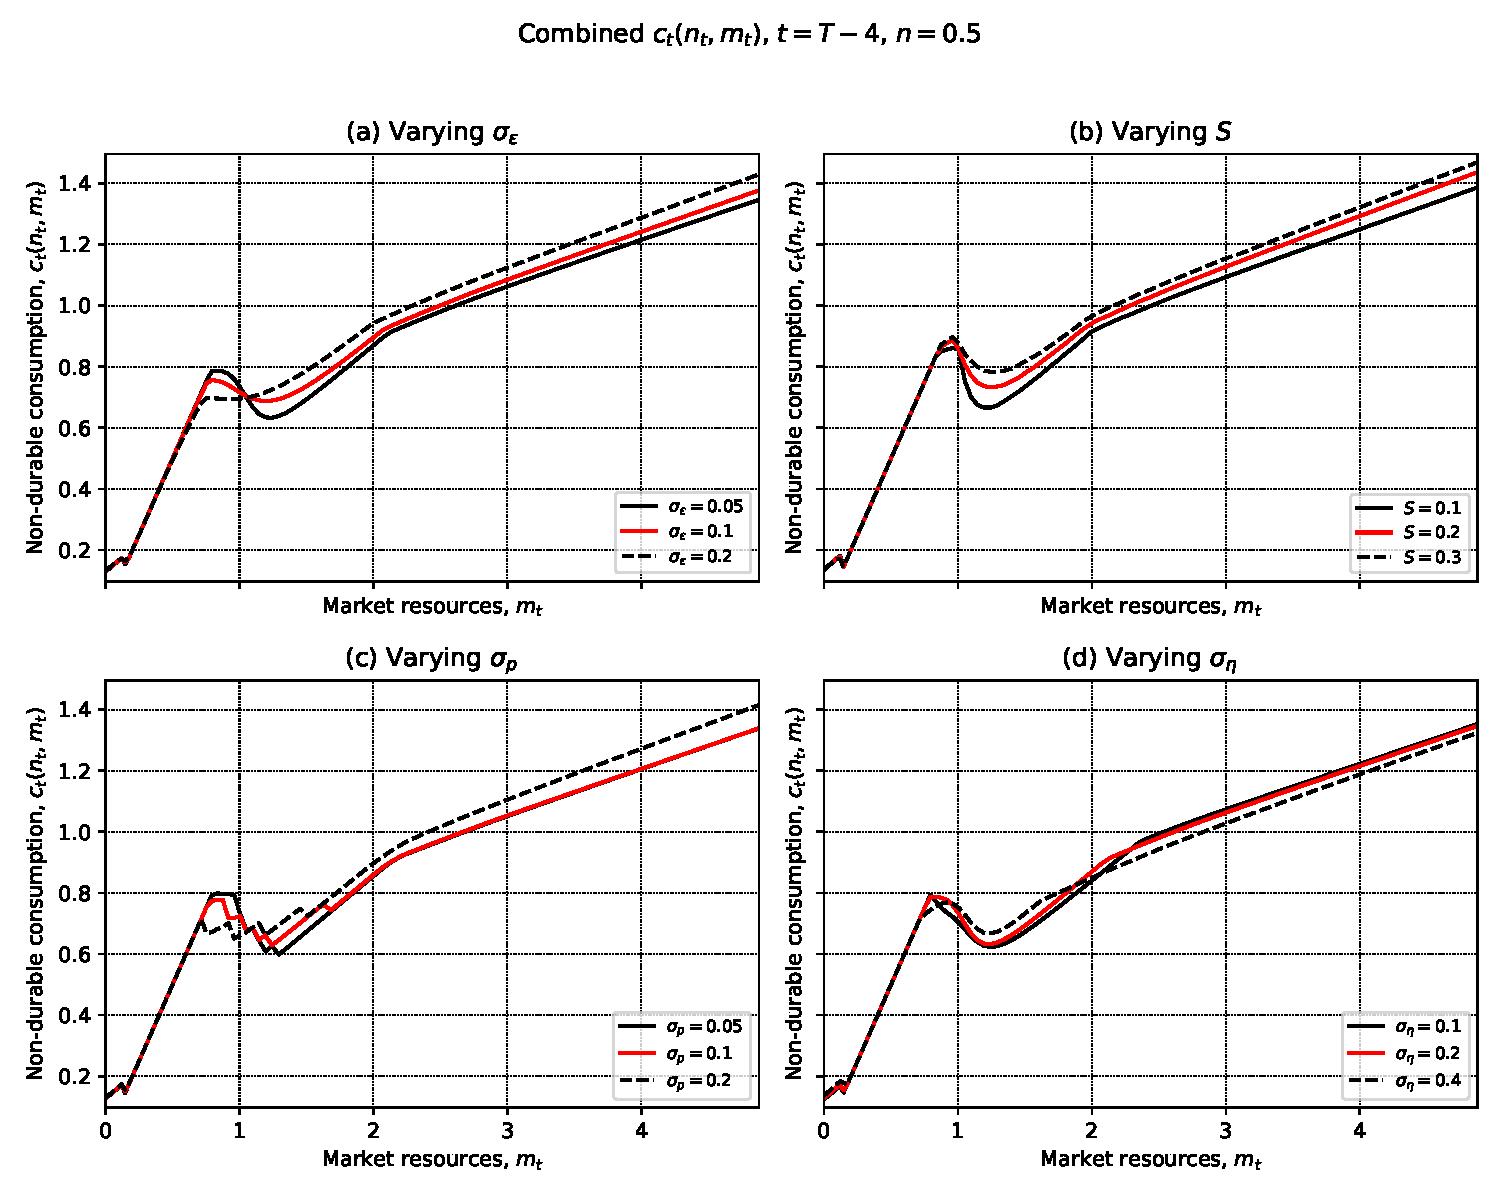
\includegraphics[width=0.78\linewidth]{SmoothingShifts_c_periodt.pdf}
	\end{center}
	\vspace{-0.15em}
	\begin{itemize}
		\item Raising $\sigma_\varepsilon$, $S$, $\sigma_p$, or $\sigma_\eta$ raises combined $c_t$ and lowers $d_t$
		\item Contrast with retirement: there taste and search shift $c$ in \emph{opposite} directions
		\item Here all reweight keep vs adjust toward less aggressive adjustment
	\end{itemize}
\end{frame}

%%% Durablemodel: Infinite Horizon: Steady state table
\begin{frame}[label = DurInfSS]
	\frametitle{Infinite horizon: steady-state aggregates}
	\vspace{-0.6em}
	{\footnotesize
	\begin{tabular}{llcccccc}
\hline
 &  & \multicolumn{6}{c}{Steady state} \\
\cline{3-8}
 &  & $C$ & $D$ & $\mathrm{DEX}$ & $\mathrm{TEX}$ & $A$ & $\mathrm{ADJ}$ (\%) \\
\hline
\multirow{3}{*}{$\sigma_\zeta$} & $0.1$ & $0.80$ & $3.56$ & $0.18$ & $0.97$ & $0.94$ & $12.2$ \\
 & $0.15$ & $0.79$ & $3.27$ & $0.16$ & $0.95$ & $0.71$ & $18.6$ \\
 & $0.2$ & $0.79$ & $3.03$ & $0.15$ & $0.94$ & $0.60$ & $24.7$ \\
\addlinespace
\multirow{3}{*}{$\sigma_p$ ($S=0.2$)} & $0.08$ & $0.81$ & $4.28$ & $0.21$ & $1.03$ & $1.39$ & $7.7$ \\
 & $0.1$ & $0.81$ & $4.51$ & $0.23$ & $1.04$ & $1.32$ & $8.7$ \\
 & $0.12$ & $0.82$ & $4.87$ & $0.24$ & $1.06$ & $1.27$ & $9.9$ \\
\addlinespace
\multirow{3}{*}{$S$ ($\sigma_p=0.1$)} & $0.15$ & $0.81$ & $4.59$ & $0.23$ & $1.04$ & $1.27$ & $9.3$ \\
 & $0.2$ & $0.81$ & $4.51$ & $0.23$ & $1.04$ & $1.32$ & $8.7$ \\
 & $0.25$ & $0.81$ & $4.45$ & $0.22$ & $1.04$ & $1.37$ & $8.3$ \\
\hline
\end{tabular}

	}
	\vspace{0.35em}
	\begin{itemize}\setlength\itemsep{0.2em}
		\item{\scriptsize Taste vs search+price: higher smoothing $\Rightarrow$ lower $C$/DEX}
		\item{\scriptsize Adjuster share: $\uparrow$ with taste or $\sigma_p$; $\downarrow$ with $S$ (given $\sigma_p$)}
	\end{itemize}
\end{frame}

%%% Durablemodel: Show Jacobians of taste shock wrt labor
\begin{frame}[label = JacTaste]
	\frametitle{Jacobians w.r.t.\ labor: taste shocks}
	\begin{center}
		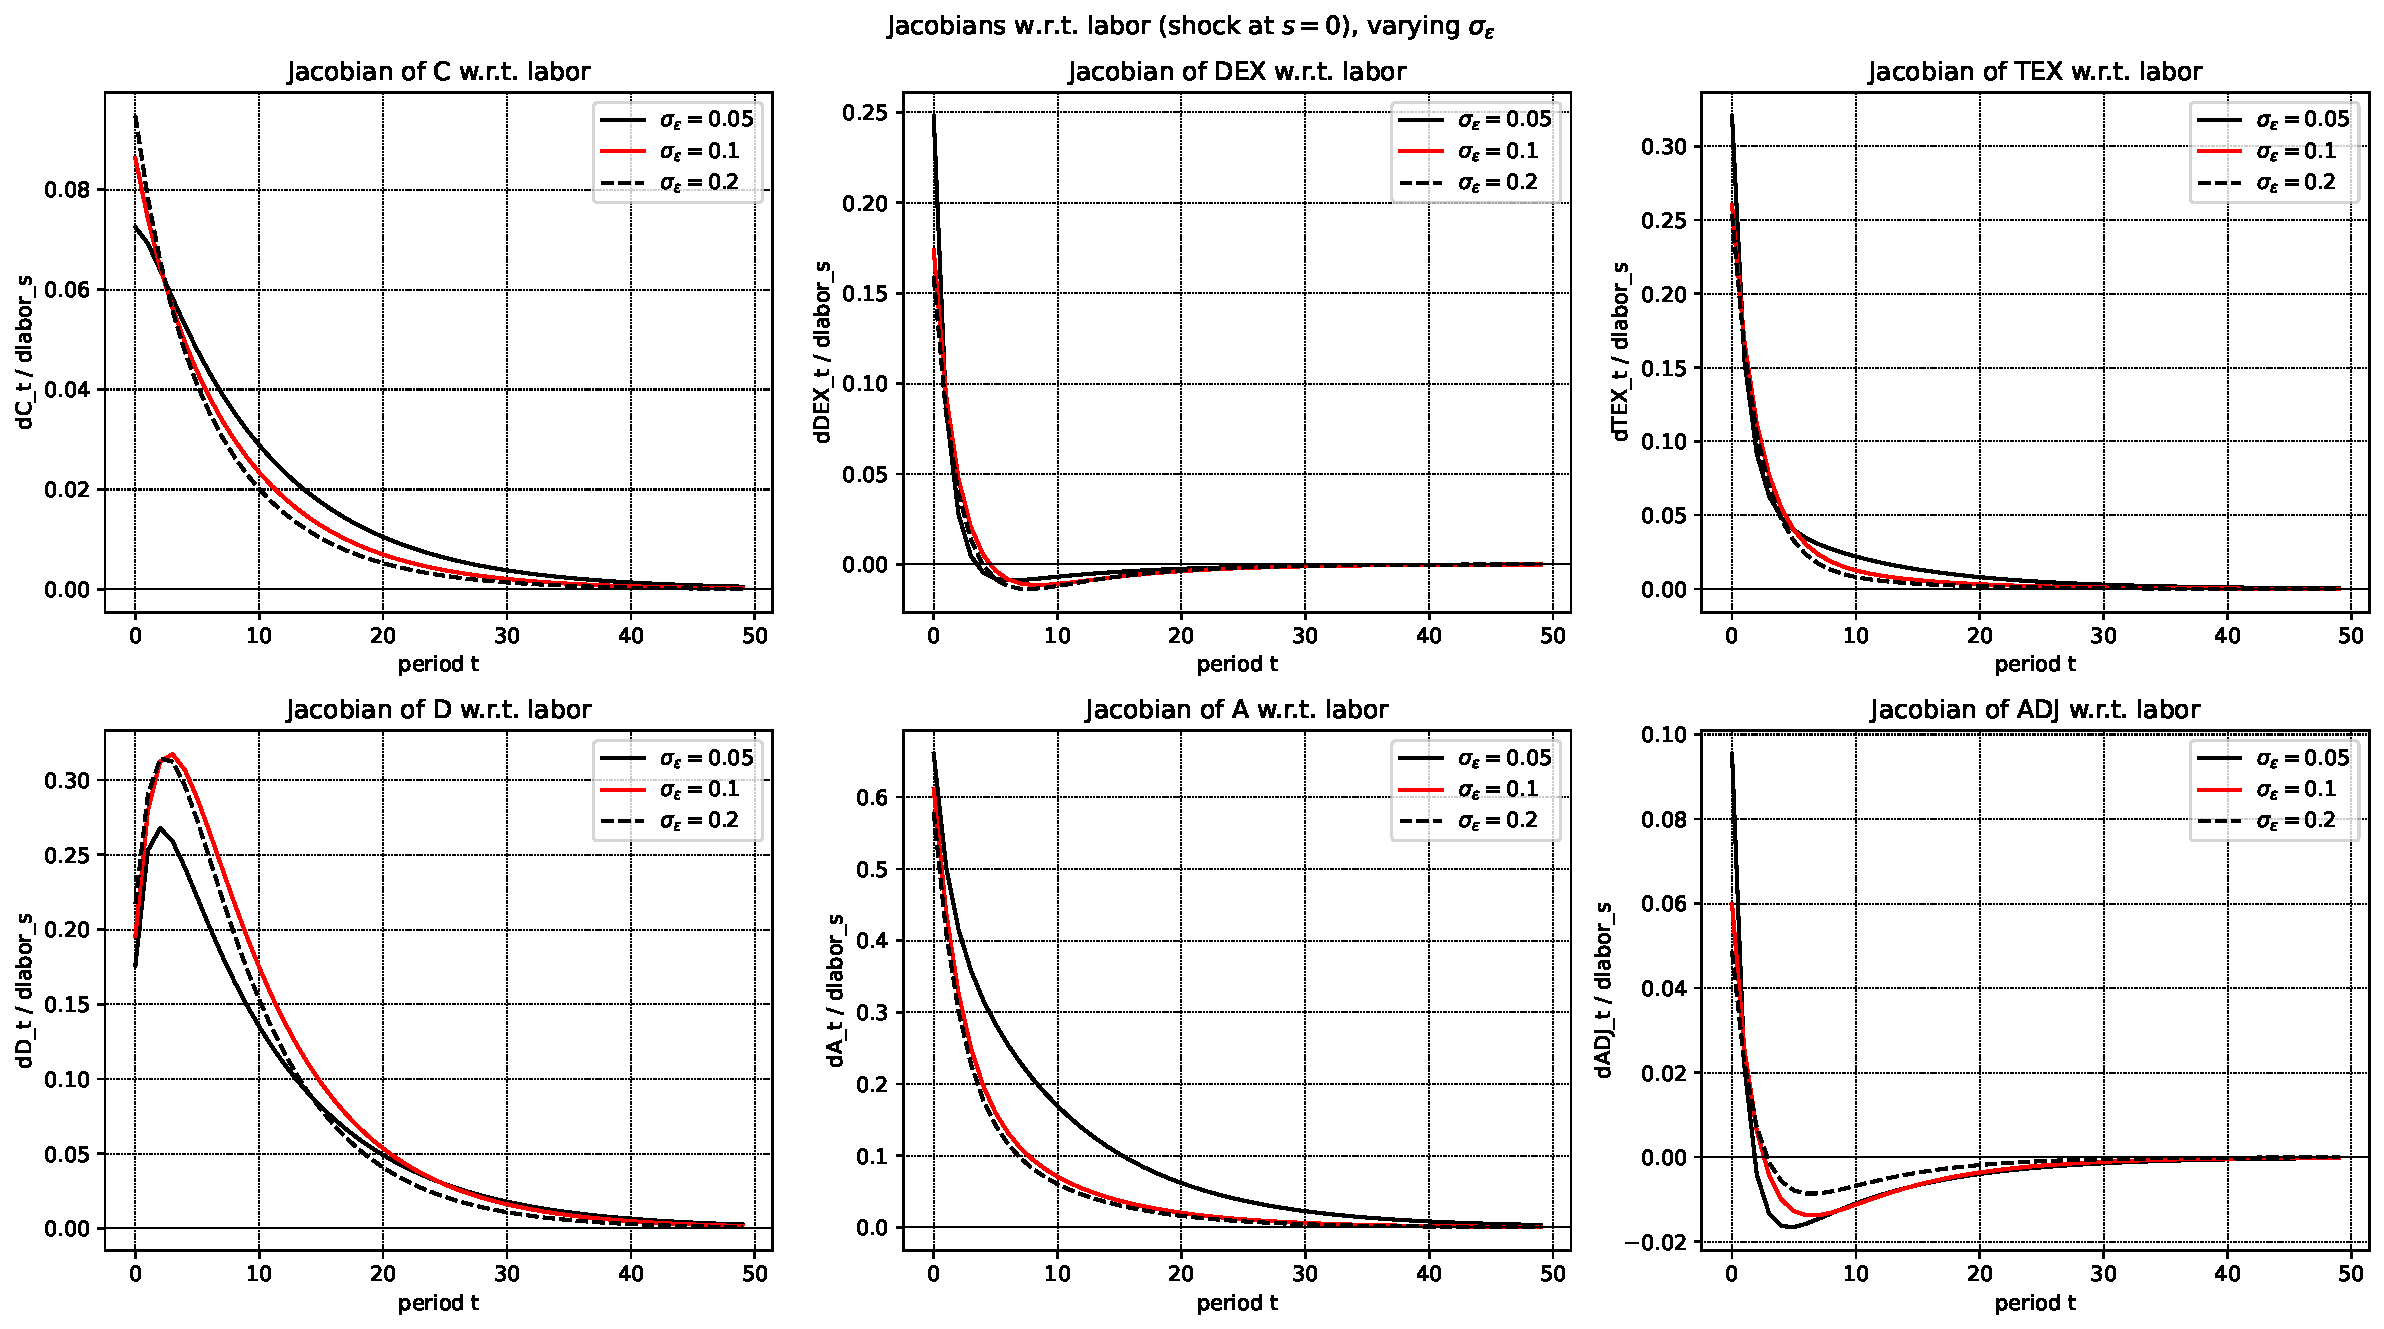
\includegraphics[width=0.82\linewidth]{Taste_Inf_Jacobians_labor.pdf}
	\end{center}
\end{frame}

%%% Durablemodel: Show Jacobians of Combined varS wrt labor
\begin{frame}[label = JacSearch]
	\frametitle{Jacobians w.r.t.\ labor: varying search intensity}
	\begin{center}
		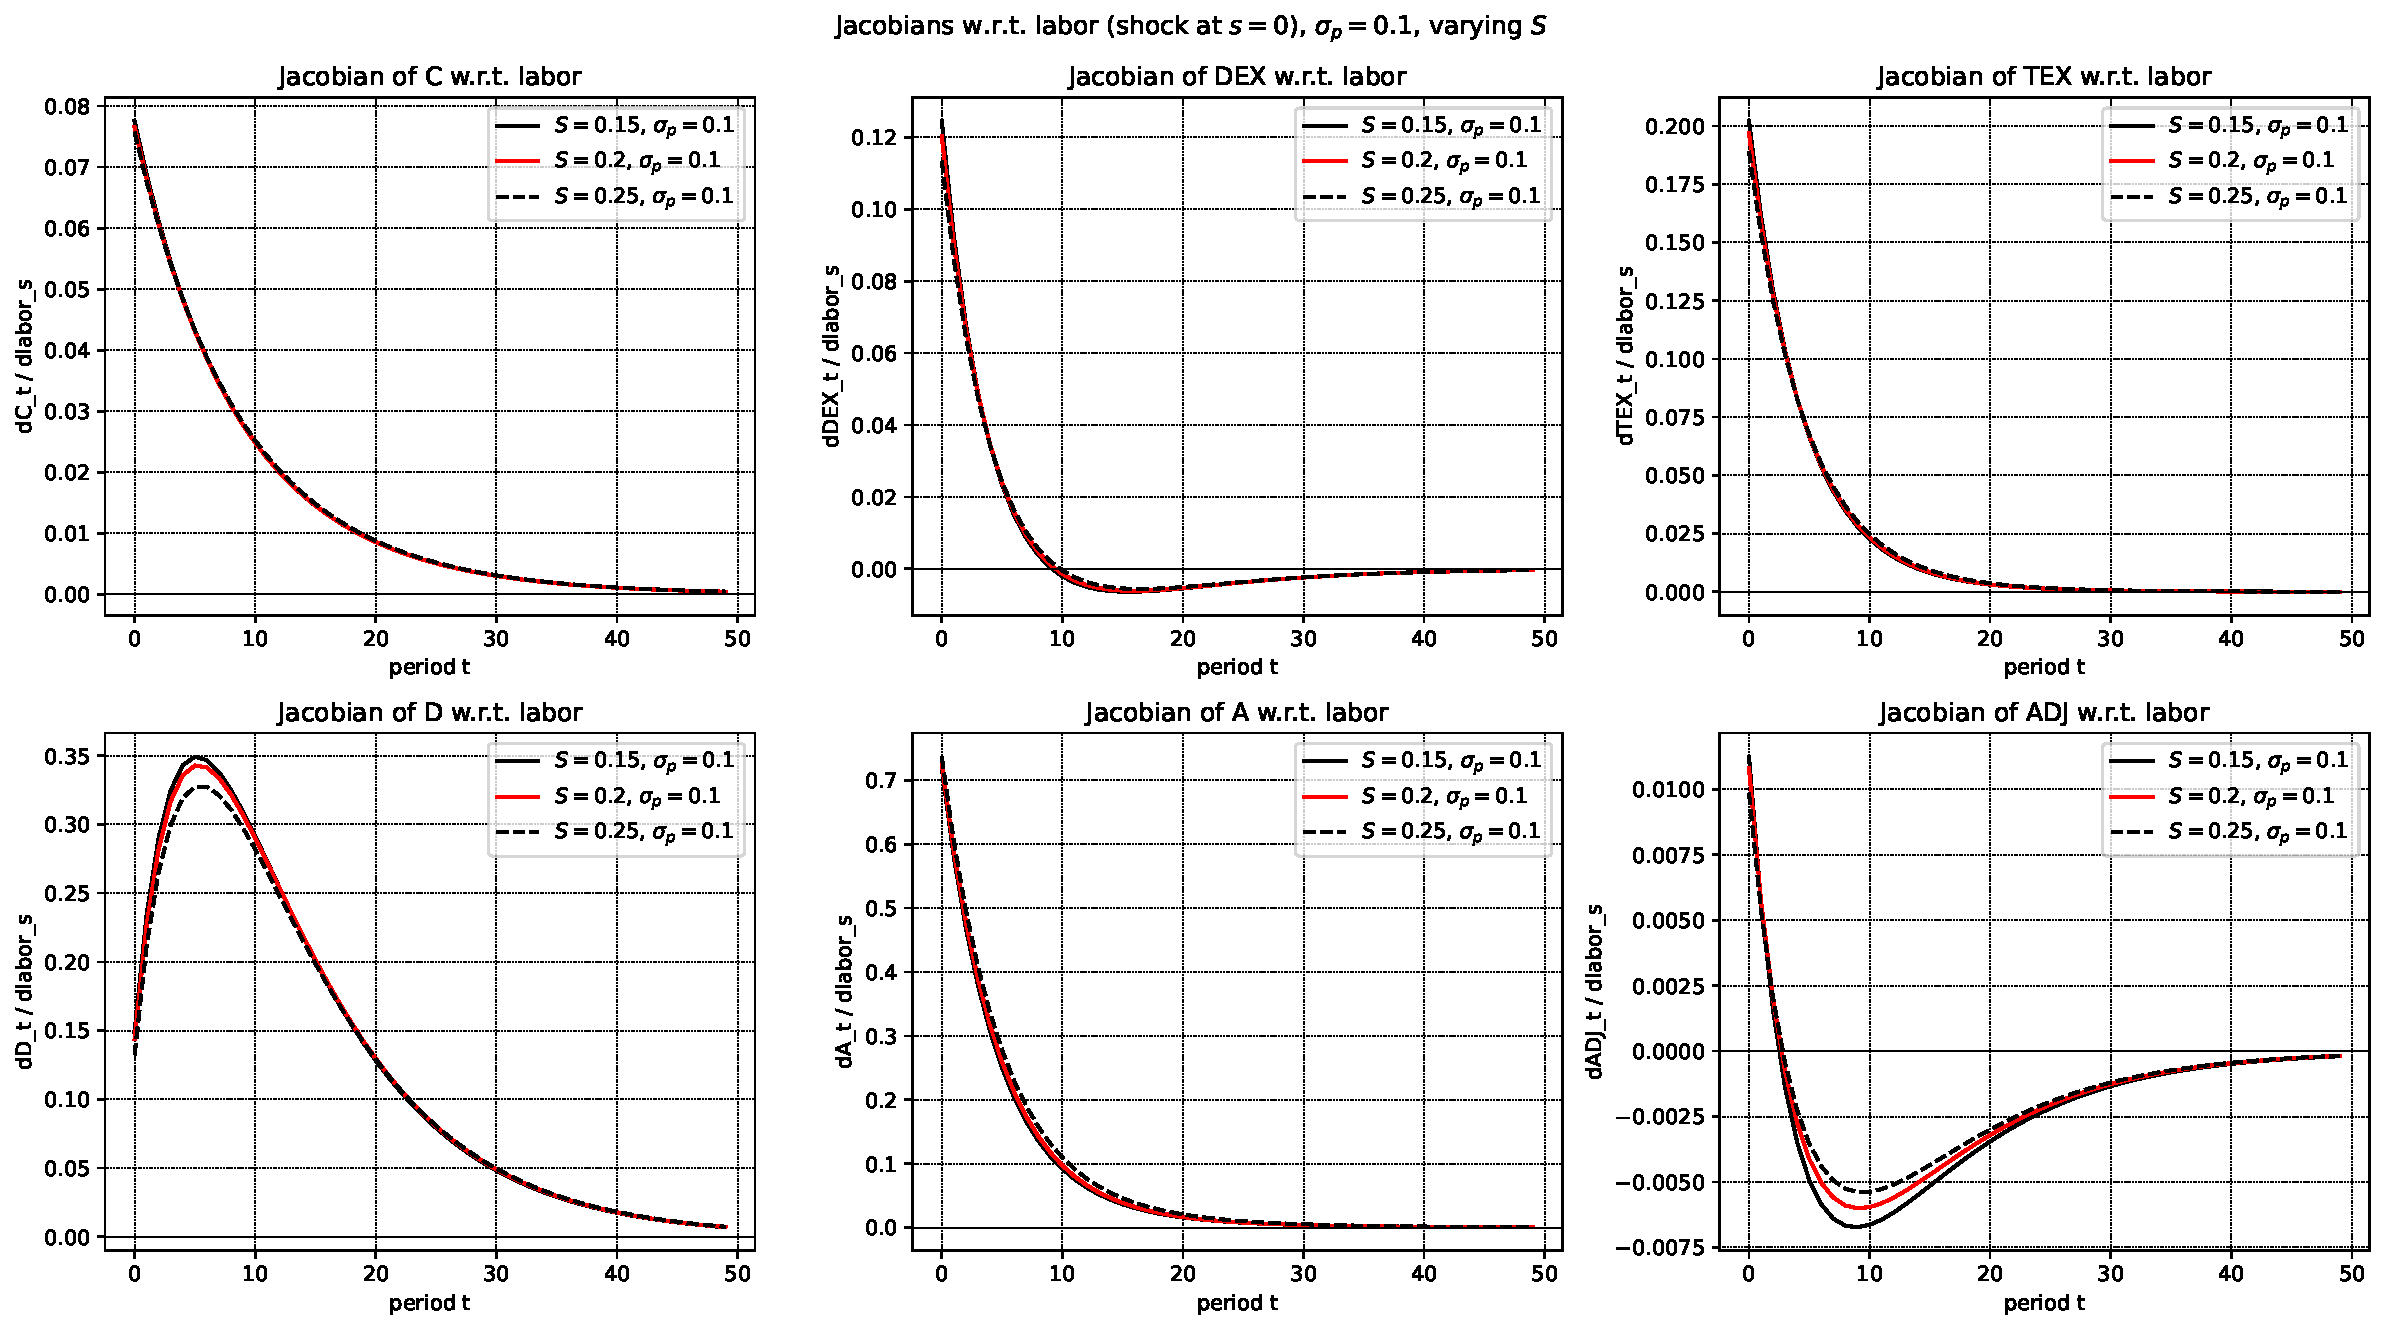
\includegraphics[width=0.82\linewidth]{Combined_varS_Inf_Jacobians_labor.pdf}
	\end{center}
\end{frame}

%%% Durablemodel: Show Jacobians of Combined varP wrt labor
\begin{frame}[label = JacPrice]
	\frametitle{Jacobians w.r.t.\ labor: varying price dispersion}
	\begin{center}
		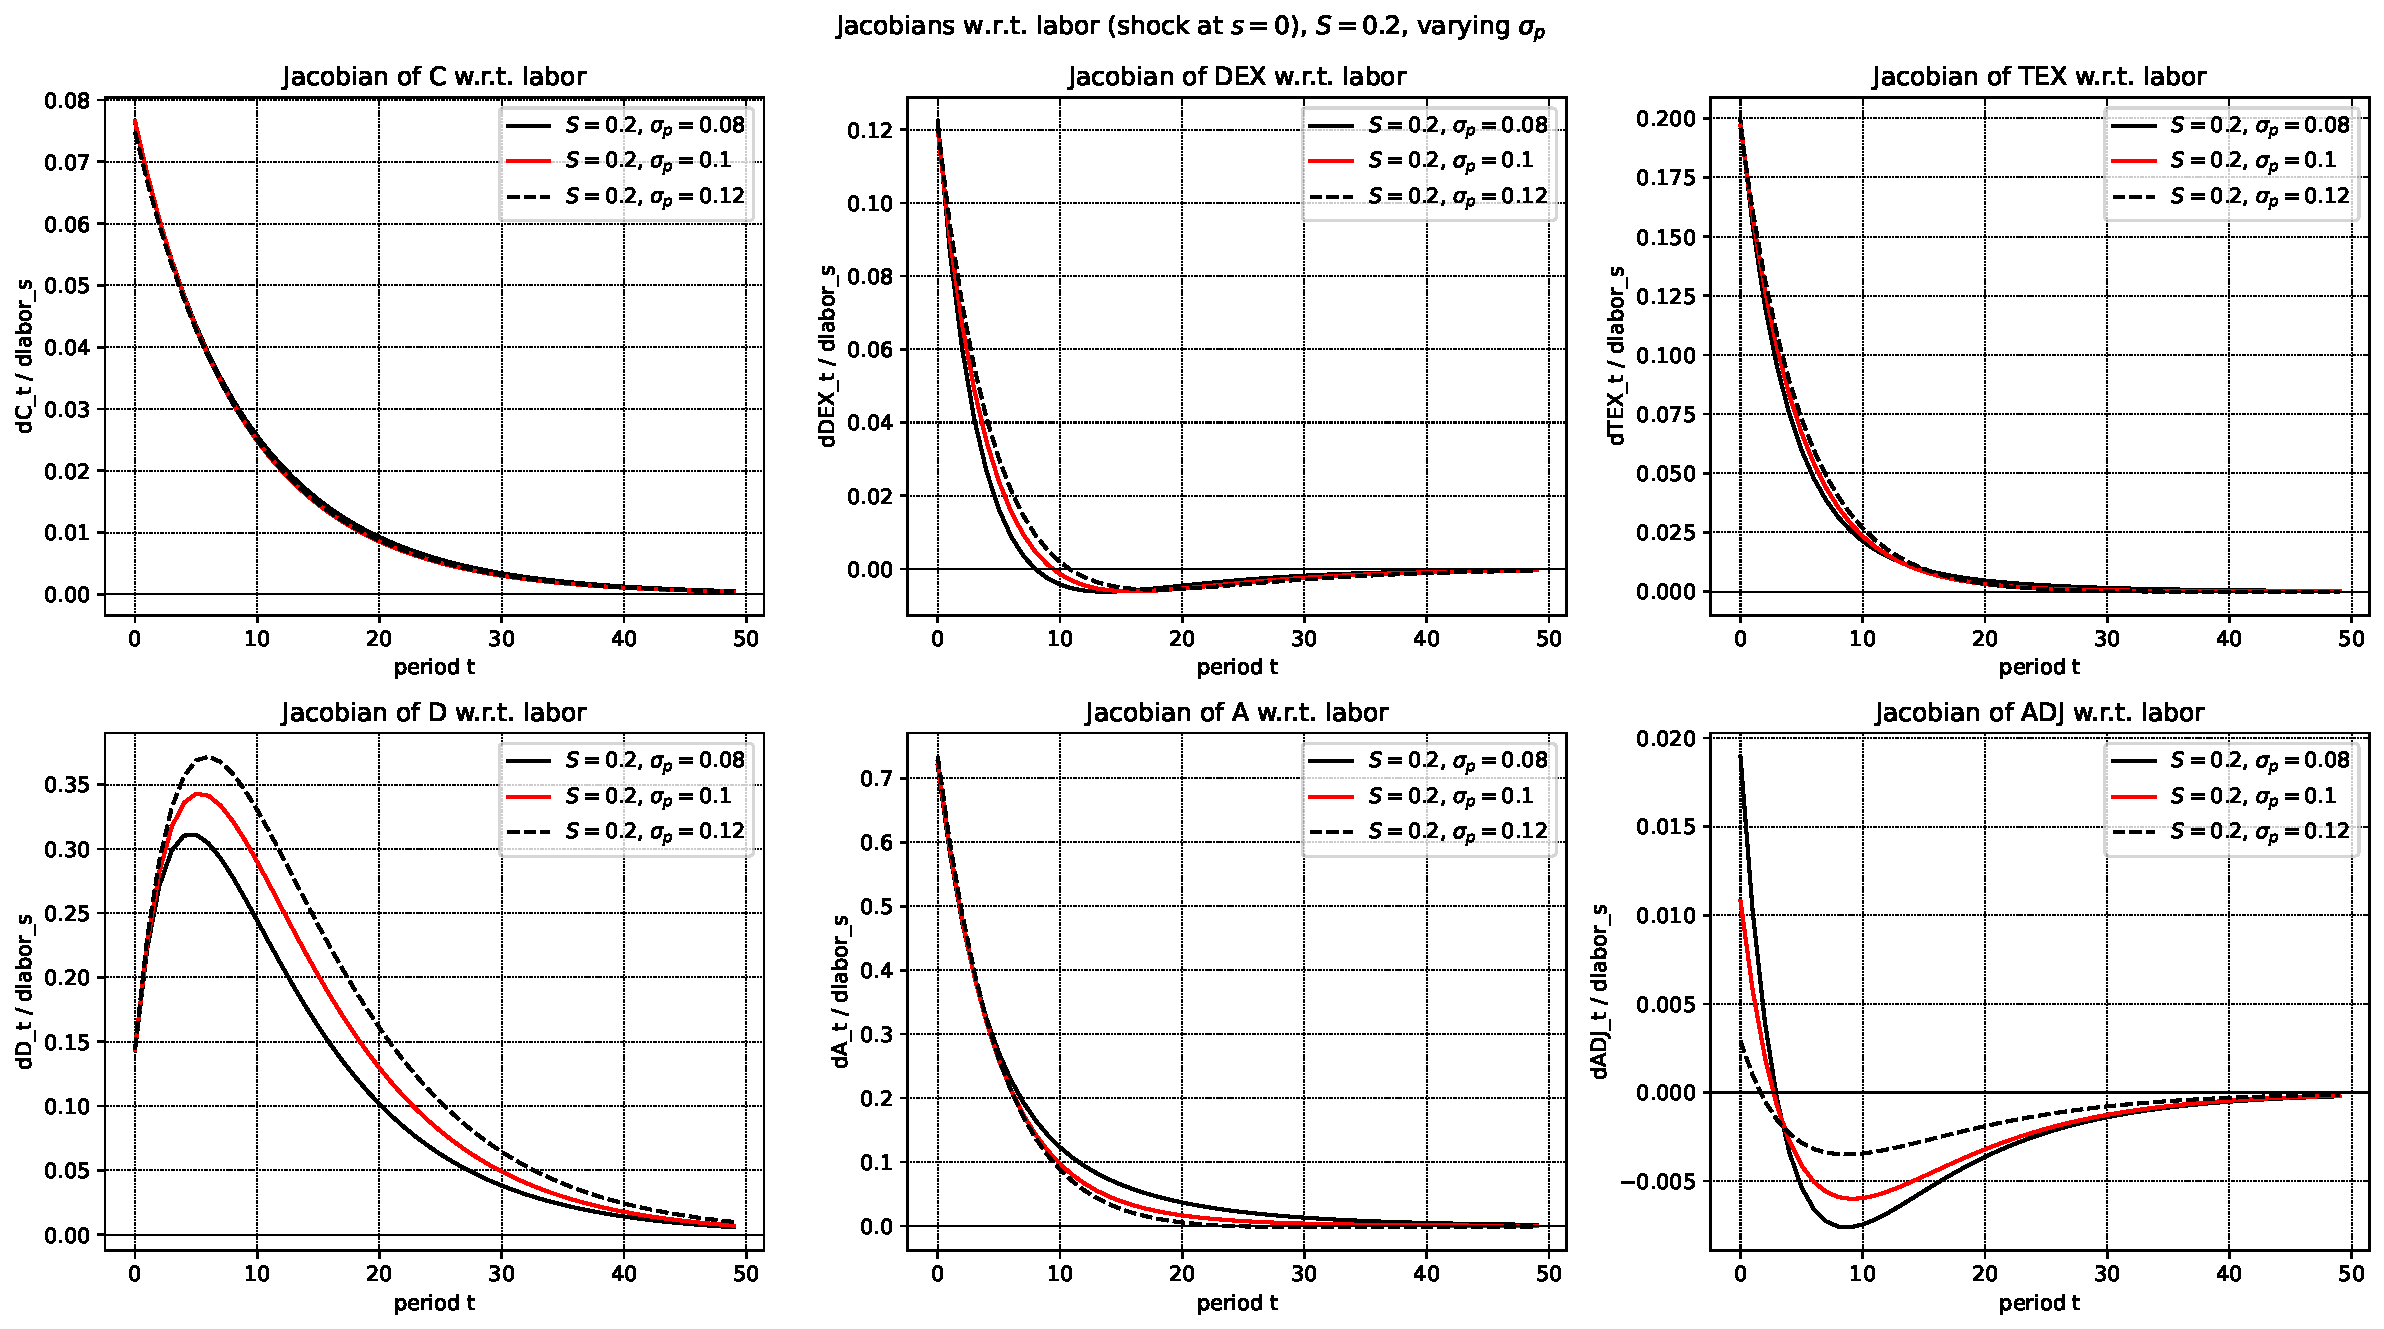
\includegraphics[width=0.82\linewidth]{Combined_varP_Inf_Jacobians_labor.pdf}
	\end{center}
\end{frame}


%============================================================
\section{Conclusion}
%============================================================

\begin{frame}[label = Conclusion]
	\frametitle{Takeaways}
	\begin{enumerate}\setlength\itemsep{0.85em}
		\item Discrete--continuous EGM produces suboptimal points from policy discontinuities
		\item Directed search + price (account) dispersion smooth those discontinuities while keeping an economic interpretation
		\item Search is preferable to taste shocks when locality, microfoundation, and PIH normalization matter
		\item In durables, all smoothers shift combined $c$ the same way; adjuster shares move differently (taste/price vs search)
		\item With enough smoothness, upper-envelope cleanup can become unnecessary
	\end{enumerate}
\end{frame}

\begin{frame}[plain]
	\centering
	\vspace{2.5em}
	{\LARGE Thank you}\\[1.5em]
	{\large Repo: \url{https://github.com/AMonninger/DCEGM_Search}}
\end{frame}

\end{document}
